\subsection{Passage du modèle Entité-Association au modèle relationnel}
Nous avions pour consigne d'utiliser un schéma Entité-Association précis et de réaliser le modèle relationnel correspondant.

\begin{figure}[H]
	\begin{center}
	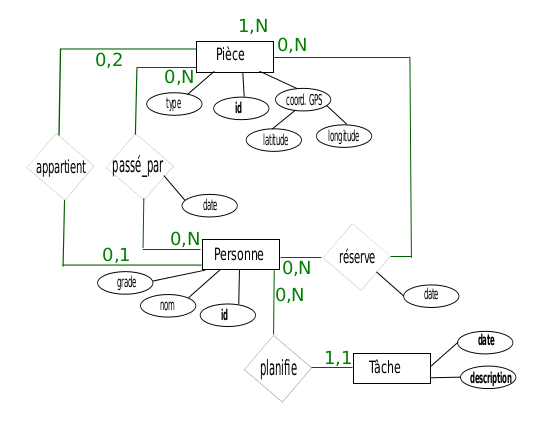
\includegraphics[width=350px]{./images/SchemaEA.png}
	\end{center}
\caption{Schéma EA}
\label{Schéma EA}
\end{figure}

En suivant chaque étape du cours, nous avons obtenu les résultats suivants :

\begin{enumerate}
	\item Passage des entités en relations :
		\begin{itemize}
			\item \code{piece}(idPiece, type, latitude, longitude) : l'attribut composite coord\_GPS est remplacé par ces 2 attributs, latitude et longitude.
			\item \code{personne}(idPers, nom, grade)
			\item \code{tache}(date, tache) 
		\end{itemize}
	\item Passage des entités faibles en relations : rien à faire puisqu'il n'y a pas d'entités faibles
	\item Association binaire 1,1 par clés étrangères :
		\begin{itemize}
			\item \code{piece}(idPiece, type, latitude, longitude) : schéma inchangé
			\item \code{personne}(idPers, nom, grade) : schéma inchangé
			\item \code{tache}(date, tache, id) : ajout de la clé étrangère idPers, clé de \code{personne} car il y a une cardinalité 1,1
		\end{itemize}
	\item Assocations binaires M,N :
		\begin{itemize}
			\item \code{piece}(idP, type, latitude, longitude) : schéma inchangé
			\item \code{personne}(idPers, nom, grade) : schéma inchangé
			\item \code{tache}(date, tache, idPers) : schéma inchangé
			\item \code{appartient}(idP, idPers) : création de la relation \code{appartient} à cette étape. Étant une table de liaison entre \code{piece} et \code{personne}, on y met les clés étrangères de ces tables. Ces seules clés permettent de modéliser la possession d'une pièce par une personne donc on n'ajoute aucun attribut. 
			\item \code{passepar}(idP, idPers, date) : création de la relation \code{passepar} à cette étape. Étant une table de liaison entre \code{piece} et \code{personne}, on y met les clés étrangères de ces tables. Nous devons ajouter un attribut \code{date} car le passage d'une personne dans une pièce doit être daté.
			\item \code{reservation}(idP, idPers, date) : création de la relation \code{reservation} à cette étape. Étant une table de liaison entre \code{piece} et \code{personne}, on y met les clés étrangères de ces tables. Nous devons ajouter un attribut \code{date} car la réservation d'une salle par une personne d'une pièce est pour une date précise.
		\end{itemize}
	\item Il n'y a pas d'attributs multi-valués ni d'association n-aire.
\end{enumerate}

\subsection{Critique du modèle Entité-Relationnel}
	On remarque que le modèle semble bien conçu et n'engendre aucun problème. Par exemple, il n'y a pas de redondance des données, les informations concernant les personnes (nom, grades) ou les pièces (coordonnées, type) ne sont pas répétées pour chaque réservation de salle avec ce modèle et le modèle relationnel qui en découle. 
	
	De ce fait, les mises à jour n'induisent pas d'incohérence : si le nom de la personne est modifié, il ne faut pas le changer à différents endroits pour rester cohérent.\\
	
	On remarque également l'absence d'anomalie de suppression. Une personne peut n'être concernée par aucune association, c'est-à-dire qu'elle ne possède pas de bureau, n'est passée par aucune pièce et n'a rien réservé, on peut tout de même conserver les informations la concernant puisqu'elles sont séparées.
